%%%%%%%%%%%%%%%%%%%%%%%%%%%%%%%%%%%%%%%%%%%%%%%%%%%%%%%%%%%%%%%%%%%%%%%%%%%%%%%
% CONTRIBUTION TO THE SURFEX BOOK2: "Land cover: ECOCLIMAP"
% Author        : S. Faroux
% Original      : January 26, 2009
% Last Update   : January 26, 2009
%%%%%%%%%%%%%%%%%%%%%%%%%%%%%%%%%%%%%%%%%%%%%%%%%%%%%%%%%%%%%%%%%%%%%%%%%%%%%%%

\chapter{Introduction}
\minitoc
%=========================
\bibliographystyle{plain}
%=========================

Ecoclimap is a global database of land surface parameters at 1-km resolution. 
It is intented to be used to initialize the soil-vegetation-atmosphere transfer schemes (SVATs) 
in meteorological and climate models. A first version was developed in 2003 (Masson \etal (2003)\nocite{masson_2003}). A second version was developed in 2008 on Europe and is implemented into Surfex. 
Ecoclimap is designed to satisfy both the Surfex "tile" approach: each grid box is made of four adjacent surfaces for nature (NAT), urban areas (TWN), sea or ocean (SEA) and lake (WAT), and the Isba "vegetation types" structure (see tab. \ref{tab1}).\\ 


\begin{table}[h]
\begin{center}
\begin{tabular}{|l|l|}
\hline
\textbf{ISBA vegetation type (vegtype)} & \textbf{abbreviation} \\
\hline
bare soil & NO \\
\hline
bare rock & ROCK \\
\hline
permanent snow & SNOW \\
\hline 
deciduous broadleaved & TREE \\
\hline
needleleaved & CONI \\
\hline
evergreen broadleaved & EVER \\
\hline
C3 crops & C3 \\
\hline
C4 crops & C4 \\
\hline
irrigated crops & IRR \\
\hline
temperate grassland & GRAS \\
\hline
tropical grassland & TROG \\
\hline
wetlands, parks and gardens & PARK \\
\hline
\end{tabular}
\end{center}
\caption{The 12 ISBA vegetation types}
\label{tab1}
\end{table}

It consists first of a global land cover map at 1/120\textdegree resolution that 
is directly read by Surfex. This map proposes a set of classes (or covers) which represent homogeneous ecosystems. 
Secondly, Surfex interprets these covers in terms of tiles and vegetation types. 
Land surface parameters (see tab. \ref{tab2a} and tab. \ref{tab2b} for the list of parameters) depend on tiles, vegetation types 
and on covers for some of them. A mechanism of aggregation 
is used to compute the surface parameters for each grid point, according to the horizontal resolution, by combining land covers defined over the 4 tiles and represented by a fraction of the 12 vegetation types (table \ref{tab1}) obtained from the 1km resolution land cover map. \\

In the first version of Ecoclimap, two hundred and fifteen ecosystems were obtained by combining existing land cover and 
climate maps, in addition to using Advanced Very High Resolution Radiometer (AVHRR) satellite data. Then, all surface parameters 
were derived for each of these ecosystems using lookup tables with the annual cycle of the leaf area index (LAI) being constrained by the AVHRR information. 
The second version uses more recent existing land cover maps. Moreover, ecosystems are now built through an automatic classification 
process applied on normalized difference vegetation index (NDVI) seven-years time series from SPOT/VEGETATION satellite data, more precise than AVHRR. Existing land cover maps give starting classes which are split in clusters by the classification process. 
Then, surface parameters are still derived using lookup tables but the annual cycle of the LAI stems from MODIS satellite data. It's possible 
to run Surfex with LAI values averaged on available years or to choose one particular year. 


\begin{table}[h]
\begin{center}
\begin{tabular}{|l|l|l| }
\hline
\textbf{surface parameter} & \textbf{abbreviation} & associated tile\\
\hline
leaf area index & LAI & nature (monthly)\\
\hline
height of trees & HT & nature \\
\hline
first soil depth & DG1 & nature\\
\hline
root depth & ROOT\_DEPTH / DG2 & nature \\
\hline
total soil depth & GROUND\_DEPTH / DG3 & nature \\
\hline
town roughness length & Z0\_TOWN & town \\
\hline
albedo of roofs,  & ALB\_ROOF, & town \\
roads, & ALB\_ROAD, &  \\
walls & ALB\_WALL &\\
\hline
emissivity of roofs,  & EMIS\_ROOF,  & town \\
roads, &  EMIS\_ROAD, & \\
walls & EMIS\_WALL & \\
\hline
heat capacity of roofs, & HC\_ROOF*3, & town \\
roads, &  HC\_ROAD*3, & \\
walls (*3 layers) &  HC\_WALL*3 & \\
\hline
thermal conductivity of roofs, & TC\_ROOF*3,  & town \\
roads, &  TC\_ROAD*3, & \\
walls (*3 layers) & TC\_WALL*3 & \\ 
\hline
width of roofs, & D\_ROOF*3,  & town \\
roads, & D\_ROAD*3, & \\
walls (*3 layers) & D\_WALL*3 & \\
\hline
buildings height & BLD\_HEIGHT & town \\
\hline
building shape & WALL\_O\_HOR & town \\
\hline
building fraction & BLD & town \\
\hline
canyons shape & CAN\_HW\_RATIO & town \\
\hline
anthropogenic sensible heat fluxes &   & town \\
due to traffic, & H\_TRAFIC, & \\
due to factory & H\_INDUSTRY & \\
\hline
anthropogenic latent heat fluxes &  & town \\ 
due to traffic, & LE\_TRAFIC,& \\
due to factory & LE\_INDUSTRY & \\
\hline
seeding date & SEED & nature \\
\hline
reaping date & REAP & nature \\
\hline
water supply quantity & WATSUP & nature \\
\hline
flag for irrigation & IRRIG & nature \\
\hline
vegetation fraction & VEG & nature (monthly)\\
\hline
dynamical vegetation  & Z0 & nature (monthly)\\
roughness length & & \\
\hline
emissivity & EMIS & nature (monthly) \\
\hline
ratio of z0 for momentum and heat & Z0\_O\_Z0H & nature  \\
\hline
\end{tabular}
\end{center}
\caption{Surface parameters given by Ecoclimap (1/2)}
\label{tab2a}
\end{table}

\begin{table}[h]
\begin{center}
\begin{tabular}{|l|l|l| }
\hline
\textbf{surface parameter} & \textbf{abbreviation} & \textbf{associated tile} \\
\hline
near infrared albedo &  ALBNIR\_VEG & nature \\
\hline
visible albedo &  ALBVIS\_VEG & nature \\
\hline
UV albedo & ALBUV\_VEG & nature \\
\hline
minimum stomatal resistance & RSMIN & nature \\
\hline
coefficient for the calculation & GAMMA & nature \\
of the surface stomatal resistance & & \\
\hline
coefficient for maximum water interception & WRMAX\_CF & nature \\
storage on capacity on the vegetation & & \\
\hline
maximum solar radiation usable in photosynthesis & RGL & nature \\
\hline
vegetation thermal intertia coefficient & CV & nature \\
\hline
mesophyll conductance & GMES, GMES\_ST & nature (AGS)\\
\hline
ecosystem respiration parameter & RE25 & nature (AGS)\\
\hline
cuticular conductance & GC, GC\_ST & nature (AGS)\\
\hline
critical normalized soil water & F2I & nature (AGS)\\
content for stress parameterisation & & \\
\hline
ratio d(biomass)/d(LAI) & BSLAI, BSLAI\_ST & nature (AGS)\\
\hline
maximum air saturation deficit & DMAX, DMAX\_ST & nature (AGS)\\
tolerated by vegetation & & \\
\hline
vegetation response type to water & STRESS & nature (AGS)\\
stress (true: defensive false: offensive) & & \\
\hline
e-folding time for senescence & SEFOLD, SEFOLD\_ST & nature (AGS)\\
\hline
minimum LAI & LAIMIN & nature (AGS)\\
\hline
leaf area ratio sensitivity & CE\_NITRO & nature (AGS)\\
to nitrogen concentration & & \\
\hline
lethal minimum value of & CF\_NITRO & nature (AGS)\\
leaf area ratio & & \\
\hline
nitrogen concentration & CNA\_NITRO & nature (AGS)\\
of active biomass & & \\
\hline
root extinction & ROOT\_EXTINCTION & nature \\
\hline
ponderation coefficient between  & ROOT\_LIN & nature \\
root fractions formulations & & \\
\hline
coefficient for SO2 deposition & SOILRC\_SO2 & nature \\
\hline
coefficient for O3 deposition & SOILRC\_O3 & nature \\
\hline
cumulative root fraction & CUM\_ROOT\_FRAC & nature \\
\hline
biomass/LAI ratio from nitrogen & BSL\_INIT\_NITRO & nature \\
declin theory & & \\
\hline
\end{tabular}
\end{center}
\caption{Surface parameters given by Ecoclimap (2/2)}
\label{tab2b}
\end{table}

\chapter{Ecoclimap characteristics}

\section{Surface parameters definition}

Parameters listed in tab. \ref{tab2a} and \ref{tab2b} are initialized: 
\begin{itemize}
\item{by cover and vegetation types for LAI, HT, DG (3 layers), SEED, REAP, WATSUP, IRRIG. Indeed, these parameters are not only a feature of 
a given vegetation type but also of regional considerations;}
\item{by vegetation type for other natural parameters. They are thus viewed as depending on the vegetation type only and not on the location; }
\item{by cover for town parameters: the "town" tile is not subdivided in types like the "nature" tile. }
\end{itemize}

Some of the natural parameters receive immediate values whereas others are calculated from some of the former. Tab. \ref{tab4a} 
and tab. \ref{tab4b} give modes of obtaining of the natural parameters (lines), by vegetation type (columns). 
Report to tab. \ref{tab1} to get the meaning of abbreviations of parameters names.\\ 
Tab \ref{tab6} delivers values for urban parameters, by type of class. 
Types of Ecoclimap urban classes come from the Corine Land Cover (CLC) classification that is considered in the two 
versions of Ecoclimap (see tab. \ref{tab5} for the correspondence).\\
All these values and formulas date from Ecoclimap-I and come from previous studies. Part of them are mentionned and detailed 
in Masson \etal (2003)\nocite{masson_2003}, other can be found in literature. 

\section{Aggregation method}

The aggregation of parameters assumes two aspects: 
\begin{itemize}
\item{the aggregation in "patchs" of several vegetation types;}
\item{the geographic aggregation linked to the spatial resolution.}
\end{itemize}
Indeed, the Surfex user can choose to work with a number of 1 to 12 patchs of vegetation types. 
Tab. \ref{tab7} gives the combinations of vegetation types according to the retained number of patches: numbers associated to vegetation types 
(columns) correspond to patchs to which they are attached, depending on the total number of patches (lines and left column). 
The Surfex user also chooses his own spatial resolution whose maximum is this of Ecoclimap: 1/120\textdegree. 
When the chosen resolution is coarser, 
parameters by grid point take aggregated values from the 1-km ones.\\ 
The common method for these two kinds of aggregation is nearly linear, apart from the fact that some particular 
averages are applied to several parameters (see tab. \ref{tab8} for more details) : 
contributions of every vegetation type to each gridpoint and each patch are weighted and added, next the total value in one point 
and one patch is brought back to the total number of contributions, that is the total weight, providing the 
wanted average value of the parameter. As seen in tab. \ref{tab9}, weights vary with parameters, depending on 
the surface on which they make sense. 

\begin{table}[htbp]
\begin{center}
\begin{tabular}{|l|l|l|l|l|l|l| }
\hline
\textbf{parameter} & \textbf{NO} & \textbf{ROCK} & \textbf{SNOW} & \textbf{TREE} & \textbf{CONI} & \textbf{EVER} \\
\hline
LAI & \multicolumn{6}{|c|}{from satellite data by cover and vegetation type} \\
\hline
HT &  \multicolumn{6}{|c|}{by cover and vegetation type} \\
\hline
DG1 & \multicolumn{6}{|c|}{by cover and vegetation type} \\
\hline
DG2 & \multicolumn{6}{|c|}{by cover and vegetation type} \\
\hline
DG3 & \multicolumn{6}{|c|}{by cover and vegetation type} \\
\hline
SEED & \multicolumn{6}{|c|}{by cover and vegetation type} \\
\hline
REAP & \multicolumn{6}{|c|}{by cover and vegetation type} \\
\hline
WATSUP & \multicolumn{6}{|c|}{by cover and vegetation type} \\
\hline
IRRIG & \multicolumn{6}{|c|}{by cover and vegetation type} \\
\hline
VEG & \multicolumn{3}{|c|}{0.} & 0.95 & 0.95 & 0.99 \\
\hline
GREEN & \multicolumn{3}{|c|}{0.}  & \multicolumn{2}{|c|}{$MIN(1-e^{-0.5*LAI},0.95)$} & 0.99 \\
\hline
Z0 & 0.1 & 1. & 0.01 & HT & HT & HT  \\
\hline
EMIS & \multicolumn{2}{|c|}{$VEG*0.97+(1-VEG)*0.94$} & 1. &  \multicolumn{3}{|c|}{$VEG*0.97+(1-VEG)*0.94$} \\
\hline
Z0\_O\_Z0H & \multicolumn{6}{|c|}{10.} \\
\hline
ALBNIR\_VEG & 0.3 & 0.3 & 0.3 & 0.25 & 0.15 & 0.21 \\
\hline
ALBVIS\_VEG & 0.1 & 0.1 & 0.1 & 0.05 & 0.05 & 0.05\\
\hline
ALBUV\_VEG & 0.06 & 0.06 & 0.06 & 0.525 & 0.0425 & 0.038 \\
\hline
RSMIN & 40. & 40. & 40. & 150. & 150. & 250. \\
\hline
GAMMA & 0. & 0. & 0. & 0.04 & 0.04 & 0.04 \\
\hline
WRMAXCF & 0.2 & 0.2 & 0.2 & 0.1 & 0.1 & 0.1 \\
\hline
RGL & 100. & 100. & 100. & 30. & 30. & 30. \\
\hline
CV & $2E^{-5}$ & $2E^{-5}$ & $2E^{-5}$ & $1E^{-5}$ & $1E^{-5}$ & $1E^{-5}$ \\
\hline
GMES & 0.02 & 0.02 & 0.02 & 0.001 & 0.001 & 0.001\\
\hline
GMES\_ST & 0.003 & 0.003 & 0.003 & 0.003 & 0.002 & 0.002 \\
\hline
RE25 & $3E^{-7}$ & $3E^{-7}$ & $3E^{-7}$ & $3E^{-7}$ & $1E^{-7}$ & $3E^{-7}$ \\
\hline
GC & 0.00025 & 0.00025 & 0.00025 & 0.00015 & 0. & 0.00015 \\
\hline
GC\_ST & 0.00015 & 0.00015 & 0.00015 & 0.00015 & 0. & 0.00015\\
\hline
F2I & 0.3 & 0.3 & 0.3 & 0.3 & 0.3 & 0.3\\
\hline
BSLAI & 0.36 & 0.36 & 0.36 & 0.25 & 0.25 & 0.25 \\ 
\hline
BSLAI\_ST & 0.08 & 0.08 & 0.08 & 0.125 & 0.50 & 0.25 \\
\hline
DMAX & 0.1 & 0.1 & 0.1 & 0.1 & 0.1 & 0.1  \\
\hline
DMAX\_ST & 0.05 & 0.05 & 0.05 & 0.109 & 0.124 & 0.124 \\
\hline
STRESS & 1. & 1. & 1. & 0. & 1. & 0. \\
\hline
SEFOLD & \multicolumn{3}{|c|}{90.*XDAY} & \multicolumn{3}{|c|}{365.*XDAY} \\
\hline
SEFOLD\_ST & \multicolumn{3}{|c|}{150.*XDAY} & 230*XDAY & \multicolumn{2}{|c|}{365.*XDAY}    \\
\hline
LAIMIN & 0.3 & 0.3 & 0.3 & 0.3 & 1. & 1.  \\ 
\hline
CE\_NITRO & 7.68 & 7.68 & 7.68 & 4.83 & 4.85 & 4.83 \\
\hline
CF\_NITRO & -4.33 & -4.33 & -4.33 & 2.53 & -0.24 & 2.53 \\
\hline
CNA\_NITRO & 1.3 & 1.3 & 1.3 & 2. & 2.8 & 2.5  \\
\hline
ROOT\_EXTINCTION & 0.961 & 0.961 & 0.961 & 0.966 & 0.943 & 0.962 \\
\hline
ROOT\_LIN & 0.05 & 0.05 & 0.05 & 0.05 & 0.05 & 0.05 \\
\hline
SOILRC\_SO2 & 1000. & 400. & 100. & 500. & 500. & 200. \\
\hline
SOILRC\_O3 & 400. & 200. & 3500. & 200. & 200. & 500.  \\
\hline
CUM\_ROOT\_FRAC & \multicolumn{6}{|c|}{$ROOT\_LIN*MIN(\frac{DG}{DG2},1.)+(1-ROOT\_LIN)*\frac{(1-ROOT\_EXT.)^{DG*100.}}{(1-ROOT\_EXT.)^{DG2*100.}}$} \\
\hline
BSL\_INIT\_NITRO & \multicolumn{6}{|c|}{$1./(CE\_NITRO+CNA\_NITRO+CF\_NITRO)$} \\
\hline
\end{tabular}
\end{center}
\caption{Lookup tables for Ecoclimap natural parameters, by vegetation type (1/2)}
\label{tab4a}
\end{table}

\begin{table}[htbp]
\begin{center}
\begin{tabular}{|l|l|l|l|l|l|l|l|l|l|l|l|l| }
\hline
\textbf{parameter} & \textbf{C3} & \textbf{C4} & \textbf{IRR} & \textbf{GRAS} & \textbf{TROG} & \textbf{PARK} \\
\hline
LAI & \multicolumn{6}{|c|}{from satellite data by cover and vegetation type} \\
\hline
HT &  \multicolumn{6}{|c|}{by cover and vegetation type} \\
\hline
DG1 & \multicolumn{6}{|c|}{by cover and vegetation type} \\
\hline
DG2 & \multicolumn{6}{|c|}{by cover and vegetation type} \\
\hline
DG3 & \multicolumn{6}{|c|}{by cover and vegetation type} \\
\hline
SEED & \multicolumn{6}{|c|}{by cover and vegetation type} \\
\hline
REAP & \multicolumn{6}{|c|}{by cover and vegetation type} \\
\hline
WATSUP & \multicolumn{6}{|c|}{by cover and vegetation type} \\
\hline
IRRIG & \multicolumn{6}{|c|}{by cover and vegetation type} \\
\hline
VEG & \multicolumn{3}{|c|}{$1-e^{-0.6*LAI}$} & 0.95 & 0.95 & 0.95 \\
\hline
GREEN & \multicolumn{3}{|c|}{$1-e^{-0.6*LAI}$} & \multicolumn{3}{|c|}{$MIN(1-e^{-0.6*LAI},0.95)$} \\
\hline
Z0 & $MIN(1.,e^{(LAI-3.5)/1.3})$ & \multicolumn{2}{|c|}{$MIN(2.5,e^{(LAI-3.5)/1.3})$} & \multicolumn{3}{|c|}{$LAI/6$} \\
\hline
EMIS & \multicolumn{6}{|c|}{$VEG*0.97+(1-VEG)*0.94$} \\
\hline
Z0\_O\_Z0H & \multicolumn{6}{|c|}{10.} \\
\hline
ALBNIR\_VEG & 0.3 & 0.3 & 0.3 & 0.3 & 0.3 & 0.3  \\
\hline
ALBVIS\_VEG & 0.1 & 0.1 & 0.1 & 0.1 & 0.1 & 0.1 \\
\hline
ALBUV\_VEG & 0.06 & 0.06 & 0.045 & 0.08 & 0.125 & 0.045 \\
\hline
RSMIN & 40. & 120. & 40. & 40. & 120. & 40. \\
\hline
GAMMA & 0. & 0. & 0. & 0. & 0. & 0. \\
\hline
WRMAXCF & 0.2 & 0.2 & 0.2 & 0.2 & 0.2 & 0.2\\
\hline
RGL & 100. & 100. & 100. & 100. & 100. & 100. \\
\hline
CV & $2E^{-5}$ & $2E^{-5}$ & $2E^{-5}$ & $2E^{-5}$ & $2E^{-5}$ & $2E^{-5}$ \\
\hline
GMES & 0.003 & 0.003 & 0.003 & 0.02 & 0.02 & 0.02 \\
\hline
GMES\_ST & 0.001 & 0.009 & 0.009 & 0.001 & 0.006 & 0.006 \\
\hline
RE25 & $3E^{-7}$ & $2.5E^{-7}$ & $3E^{-7}$ & $3E^{-7}$ & $3E^{-7}$ & $3E^{-7}$ \\
\hline
GC & 0.00025 & 0.00025 & 0.00025 & 0.00025 & 0.00025 & 0.00025  \\
\hline
GC\_ST & 0.00025 & 0.00015 & 0.00015 & 0.00025 & 0.00015 & 0.00025 \\
\hline
F2I & 0.3 & 0.3 & 0.3 & 0.3 & 0.3 & 0.3 \\
\hline
BSLAI & 0.06 & 0.06 & 0.06 & 0.36 & 0.36 & 0.36\\ 
\hline
BSLAI\_ST & 0.06 & 0.06 & 0.06 & 0.08 & 0.08 & 0.08\\
\hline
DMAX & 0.1 & 0.1 & 0.1 & 0.1 & 0.1 & 0.1 \\
\hline
DMAX\_ST & 0.05 & 0.033 & 0.033 & 0.05 & 0.052 & 0.05 \\
\hline
STRESS & 1. & 0. & 1. & 0. & 0. & 0. \\
\hline
SEFOLD & \multicolumn{3}{|c|}{60.*XDAY} & \multicolumn{3}{|c|}{90.*XDAY} \\
\hline
SEFOLD\_ST & \multicolumn{6}{|c|}{150.*XDAY} \\
\hline
LAIMIN & 0.3 & 0.3 & 0.3 & 0.3 & 0.3 & 0.3 \\ 
\hline
CE\_NITRO & 3.79 & 7.68 & 7.68 & 5.56 & 7.68 & 5.56 \\
\hline
CF\_NITRO & 9.84 & -4.33 & -4.33 & 6.73 & -4.33 & 6.73 \\
\hline
CNA\_NITRO & 1.3 & 1.9 & 1.9 & 1.3 & 1.3 & 1.3  \\
\hline
ROOT\_EXTINCTION & 0.961 & 0.972 & 0.961 & 0.943 & 0.972 & 0.943 \\
\hline
ROOT\_LIN & 0.05 & 0.05 & 0.05 & 0.05 & 0.5 & 0.5 \\
\hline
SOILRC\_SO2 & 150. & 150. & 0.001 & 350. & 350. & 100.  \\
\hline
SOILRC\_O3 & 150. & 150. & 1000. & 200. & 200. & 700.  \\
\hline
CUM\_ROOT\_FRAC & \multicolumn{6}{|c|}{$ROOT\_LIN*MIN(\frac{DG}{DG2},1.)+(1-ROOT\_LIN)*\frac{(1-ROOT\_EXT.)^{DG*100.}}{(1-ROOT\_EXT.)^{DG2*100.}}$} \\
\hline
BSL\_INIT\_NITRO & \multicolumn{6}{|c|}{$1./(CE\_NITRO+CNA\_NITRO+CF\_NITRO)$} \\
\hline
\end{tabular}
\end{center}
\caption{Lookup tables for Ecoclimap natural parameters, by vegetation type (2/2)}
\label{tab4b}
\end{table}


\begin{table}[htbp]
\begin{center}
\begin{tabular}{|l|l|l|l|l|l|l|l|l|l| }
\hline
\textbf{parameter} & \textbf{151} & \textbf{152} & \textbf{155} & \textbf{156} & \textbf{157} & \textbf{158} & \textbf{159} & \textbf{160} & \textbf{161} \\
\hline
ALB\_ROOF & \multicolumn{9}{|c|}{0.15} \\
\hline
ALB\_ROAD &  \multicolumn{9}{|c|}{0.25} \\
\hline
ALB\_WALL & \multicolumn{9}{|c|}{0.08} \\
\hline
EMIS\_ROOF & \multicolumn{9}{|c|}{0.90} \\ 
\hline
EMIS\_ROAD & \multicolumn{9}{|c|}{0.94} \\
\hline
EMIS\_WALL & \multicolumn{9}{|c|}{0.85} \\
\hline
HC\_ROOF(1) &  \multicolumn{9}{|c|}{$2.11E^{6}$} \\
\hline
HC\_ROOF(2) &  \multicolumn{9}{|c|}{$0.28E^{6}$} \\
\hline
HC\_ROOF(3) &  \multicolumn{9}{|c|}{$0.29E^{6}$} \\
\hline
HC\_ROAD(1) &  \multicolumn{9}{|c|}{$1.94E^{6}$} \\
\hline
HC\_ROAD(2) &  \multicolumn{9}{|c|}{$1.28E^{6}$} \\
\hline
HC\_ROAD(3) &  \multicolumn{9}{|c|}{$1.28E^{6}$} \\
\hline
HC\_WALL(1) &  \multicolumn{9}{|c|}{$1.55E^{6}$} \\
\hline
HC\_WALL(2) &  \multicolumn{9}{|c|}{$1.55E^{6}$} \\
\hline
HC\_WALL(3) &  \multicolumn{9}{|c|}{$0.29E^{6}$} \\
\hline
TC\_ROOF(1) &  \multicolumn{9}{|c|}{1.51} \\
\hline
TC\_ROOF(2) &  \multicolumn{9}{|c|}{0.08} \\
\hline
TC\_ROOF(3) &  \multicolumn{9}{|c|}{0.05} \\
\hline
TC\_ROAD(1) &  \multicolumn{9}{|c|}{0.7454} \\
\hline
TC\_ROAD(2) &  \multicolumn{9}{|c|}{0.2513} \\
\hline
TC\_ROAD(3) &  \multicolumn{9}{|c|}{0.2513} \\
\hline
TC\_WALL(1) &  \multicolumn{9}{|c|}{0.9338} \\
\hline
TC\_WALL(2) &  \multicolumn{9}{|c|}{0.9338} \\
\hline
TC\_WALL(3) &  \multicolumn{9}{|c|}{0.05} \\
\hline
D\_ROOF(1) &  \multicolumn{9}{|c|}{0.05} \\
\hline
D\_ROOF(2) &  \multicolumn{9}{|c|}{0.4} \\
\hline
D\_ROOF(3) &  \multicolumn{9}{|c|}{0.1} \\
\hline
D\_ROAD(1) &  \multicolumn{9}{|c|}{0.05} \\
\hline
D\_ROAD(2) &  \multicolumn{9}{|c|}{0.1} \\
\hline
D\_ROAD(3) &  \multicolumn{9}{|c|}{1.} \\
\hline
D\_WALL(1) &  \multicolumn{9}{|c|}{0.02} \\
\hline
D\_WALL(2) &  \multicolumn{9}{|c|}{0.125} \\
\hline
D\_WALL(3) &  \multicolumn{9}{|c|}{0.05} \\
\hline
Z0\_TOWN & 3. & 1. & 2. & 0.5 & 2. & 0.01 & 0.1 & 0.5 & 1. \\
\hline 
BLD\_HEIGHT & 30. & 10. & 20. & 5. & 20. & 10. & 5. & 5. & 10. \\
\hline
WALL\_O\_HOR & 1. & 0.5 & 0.5 & 0.5 & 1. & 0.5 & 0.5 & 0.5 & 1. \\
\hline
BLD & 0.5 & 0.5 & 0.5 & 0.1 & 0.5 & 0.1 & 0.1 & 0.1 & 0.5 \\
\hline
CAN\_HW\_RATIO & \multicolumn{9}{|c|}{$0.5*\frac{WALL\_O\_HOR}{1-BLD}$} \\
\hline
H\_TRAFIC & 20 & 10. & 10. & 30. & 10. & 10. & 0. & 0. & 0. \\
\hline
H\_INDUSTRY & 10. & 5. & 20. & 0. & 20. & 0. & 0. & 0. & 0. \\
\hline
LE\_TRAFIC & 0. & 0. & 0. & 0. & 0. & 0. & 0. & 0. & 0. \\
\hline
LE\_INDUSTRY & 0. & 0. & 0. & 0. & 0. & 0. & 0. & 0. & 0. \\
\hline
\end{tabular}
\end{center}
\caption{Lookup tables for Ecoclimap urban parameters, by cover}
\label{tab6}
\end{table}

\begin{table}[htbp]
\begin{center}
\begin{tabular}{|l|l| }
\hline
\textbf{cover name} & \textbf{cover(s) number(s)} \\
\hline
dense urban & 151 \\
\hline 
suburban & 152,153,154,7 \\
\hline
industries and commercial areas & 155 \\
\hline
road and rail networks & 156 \\
\hline
port facilities & 157 \\
\hline
airport & 158 \\
\hline
mineral extraction and construction sites & 159 \\
\hline
urban parks & 160 \\
\hline
sport facilities & 161 \\
\hline
\end{tabular}
\end{center}
\caption{Ecoclimap covers numbers for urban classes}
\label{tab5}
\end{table}

\begin{table}[htbp]
\begin{center}
\begin{tabular}{|l|l|l|l|l|l|l|l|l|l|l|l|l|}
\hline
\textbf{patchs} & \textbf{NO} & \textbf{ROCK} & \textbf{SNOW} & \textbf{TREE} & \textbf{CONI} & \textbf{EVER} & \textbf{C3} & \textbf{C4} & \textbf{IRR} & \textbf{GRAS} & \textbf{TROG} & \textbf{PARK} \\
\hline
\textbf{1} & 1 & 1 & 1 & 1 & 1 & 1 & 1 & 1 & 1 & 1 & 1 & 1 \\
\hline
\textbf{2} & 1 & 1 & 1 & 2 & 2 & 2 & 1 & 1 & 1 & 1 & 1 & 1 \\
\hline
\textbf{3} & 1 & 1 & 1 & 2 & 2 & 2 & 3 & 3 & 3 & 3 & 3 & 3 \\
\hline
\textbf{4} & 1 & 1 & 1 & 2 & 2 & 2 & 3 & 3 & 3 & 4 & 4 & 4 \\
\hline
\textbf{5} & 1 & 1 & 1 & 2 & 2 & 2 & 3 & 3 & 4 & 5 & 5 & 4 \\
\hline
\textbf{6} & 1 & 1 & 1 & 2 & 2 & 2 & 3 & 3 & 4 & 5 & 5 & 6 \\
\hline
\textbf{7} & 1 & 1 & 2 & 3 & 3 & 3 & 4 & 4 & 5 & 6 & 6 & 7 \\
\hline
\textbf{8} & 1 & 1 & 2 & 3 & 3 & 3 & 4 & 5 & 6 & 7 & 7 & 8 \\
\hline
\textbf{9} & 1 & 1 & 2 & 3 & 4 & 3 & 5 & 6 & 7 & 8 & 8 & 9 \\
\hline
\textbf{10} & 1 & 1 & 2 & 3 & 4 & 5 & 6 & 7 & 8 & 9 & 9 & 10 \\
\hline
\textbf{11} & 1 & 2 & 3 & 4 & 5 & 6 & 7 & 8 & 9 & 10 & 10 & 11 \\
\hline
\textbf{12} & 1 & 2 & 3 & 4 & 5 & 6 & 7 & 8 & 9 & 10 & 11 & 12 \\
\hline
\end{tabular}
\end{center}
\caption{Combinations of vegetation types according to the retained number of patchs in Surfex}
\label{tab7}
\end{table}

\begin{table}[htbp]
\begin{center}
\begin{tabular}{|l|l|l|l|l|}
\hline
\textbf{averaging type} & \textbf{name} & \textbf{added element} & \textbf{averaging} & \textbf{affected parameters} \\
\hline
ARI & arithmetic & $X$ & $\Sigma/\Gamma$ & every but... \\
\hline
INV & inverse & $1./X$ & $\Gamma/\Sigma$ & RSMIN, CV, HC\_ROOF, \\
 & & & & HC\_ROAD, HC\_WALL\\
\hline
CDN & inverse of  & $1./LN(DZ/X)^2$ & $DZ*e^{-\sqrt{\Gamma/\Sigma}}$ & Z0, Z0\_TOWN \\
 &square & with $DZ$ height of the &  & \\
 & logarithm & first model mass level if &  & \\
 & & available and 20m otherwise & &  \\
\hline
MAJ & dominant & no addition: the most & none &  SEED, REAP \\
  &  date & frequently occurrent& & \\
  &  &  date is selected & & \\
\hline
\end{tabular}
\end{center}
\caption{Averaging types and associated parameters in Ecoclimap. $X$ is a single value of the parameter to average; 
$\Sigma$ represents the total  
of the added weighted elements; $\Gamma$ represents the total weight of the added weighted elements. }
\label{tab8}
\end{table}


\begin{table}[h]
\begin{center}
\begin{tabular}{|l|l|l|l|}
\hline
\textbf{type of weight} & \textbf{name} & \textbf{value} & \textbf{associated parameters} \\
\hline
ALL & all & 1. & fractions of tiles \\
 & & & NAT,TWN,SEA,WAT \\
\hline
NAT & nature & fraction of tile "nature" & fractions of vegtypes,  \\
 & & (* fraction of added vegtype) & VEG, Z0, Z0\_O\_Z0H, EMIS, \\
 & & & DG, CUM\_ROOT\_FRAC, RE25\\
\hline
TRE & tree & fraction of tile "nature" & HT, DMAX\_ST, DMAX\\
 & & * (either) fraction of vegtype TREE & \\
 & & *(or) fraction of vegtype CONI & \\
 & & *(or) fraction of vegtype EVER & \\
 & & (non-zero only for trees vegtypes) &\\
\hline
LAI & LAI & fraction of tile "nature" & RSMIN\\
 & & * fraction of added vegtype & \\
 & & * associated LAI value & \\
\hline
VEG & fraction of& fraction of tile "nature" & all remaining \\
 &  vegetation & * fraction of added vegtype &  natural parameters \\
 & & * associated VEG value &\\
\hline
TWN & town & fraction of tile "town" & every town parameter but... \\
\hline
BLD & building & fraction of tile "town" & ALB\_ROOF, EMIS\_ROOF, HC\_ROOF, \\
 & & * fraction of building BLD &  TC\_ROOF, D\_ROOF, ALB\_WALL, \\
 & & & EMIS\_WALL, HC\_WALL, TC\_WALL, \\
 & & & D\_WALL, WALL\_O\_HOR \\
\hline
STR & street & fraction of tile "town" & ALB\_ROAD, EMIS\_ROAD, \\
 & & * (1.-fraction of building BLD) & HC\_ROAD, TC\_ROAD, \\
 & & & D\_ROAD\\
\hline
\end{tabular}
\end{center}
\caption{Weighting functions and associated parameters in Ecoclimap. Parenthesis indications in the "value" column refer to 
what happens in case of calculation defined by patch, ie for all natural parameters but neither for the fractions of tiles and 
vegetation types nor for the town parameters.}
\label{tab9}
\end{table}


\section{Writing of parameters in a latex file}

Distribution of classes among tiles and vegetation types, also values of surface parameters are described in a tex file called \textit{class\_cover\_data.tex}. 
It can be compiled to get a ps or pdf file that recapitulates all these values in different arrays. 

\chapter{Ecoclimap-II realization}

Ecoclimap-II has been developed on a European field. Its limits are 11W and 62E in longitude and 25N and 75N in latitude. 

\section{The Ecoclimap-II map}

\subsection{The initial map}\label{init_map}

Existing land cover maps taken into account in this development are:
\begin{itemize}
\item{Global Land Cover 2000 (GLC2000)\footnote{http://www-gvm.jrc.it/glc2000};}
\item{Corine Land Cover 2000 (CLC2000)\footnote{http://www.ifen.fr, http://www.eea.eu.int};}
\end{itemize}
GLC2000 was built from daily SPOT/VEGETATION satellite data for year 2000 (dataset VEGA2000). The spatial resolution is 1/112\textdegree~(corresponding to $\sim$1.1km) and 
the projection is latlon. Several regional maps and a global map of 23 classes exist. The latter global map 
is taken as a basis and classes from available regional maps are added when relevant. \\
Then, CLC2000 covers only a part of the domain (political Europe) and includes 44 classes. 
It was realized by photo-interpretation of SPOT and LANDSAT satellite images. The projection 
is Lambert's azimuthal equivalent and the resolution is 100m. In order to fit Ecoclimap, 
Corine data are reprojected and brought back to the 
same resolution. In these conditions, the Corine class number attributed to the pixel at 1-km resolution is this of the most numerous class into the pixel. It's decided to introduce majority classes at more than 70\% in the map under construction. It happens that 55\% of Corine pixels are 
kept by this way. So-obtained Corine pixels have priority on GLC information because their contents is better known and supposed to characterize 
more homogeneous ecosystems. \\
The resulting map comprises classes from several origins and potentially complementary: their headings 
and geographic distribution give indications to melt some of them. 
After a couple of such combinations, a 76-covers map (called \textbf{C76} from now on) is finally 
obtained on the considered area. This map is the reference used for the further classification process. 
It's thus a mix of GLC2000 and CLC2000.  

\subsection{NDVI satellite data}\label{ndvi}


NDVI is deduced from B2 (red) and B3 (near infrared) satellite normalized reflectances (ratios of the reflected over the incoming radiation 
in each spectral band) 
according to the formula: 
\begin{displaymath}
NDVI=\frac{B3-B2}{B3+B2}~~~~~~(1)
\end{displaymath}
This rate usually ranges from 0 to 1. Negative values indicate the presence of snow. Works have shown a correlation between NDVI values and the 
vegetation photosynthesis activity. The LAI and NDVI annual cycles are supposed to be correlated. In Ecoclimap-I, 
LAI profiles by cover were obtained from NDVI through the formula: 
\begin{displaymath}
LAI(t)=LAI_{min}+(LAI_{max}-LAI_{min})*\frac{NDVI(t)-NDVI_{min}}{NDVI_{max}-NDVI_{min}}~~~~~~(2)
\end{displaymath} 
$LAI_{min}$ and $LAI_{max}$ being set from in-situ measurements or empirically following ISBA simulations. Then, LAI profiles by vegetation types 
(inside covers) are deduced from these LAI by cover thanks to simple rules, mostly by changing extreme values of the cycle ($LAI_{min}$ and $LAI_{max}$) 
depending on the vegetation height in the formula (2), sometimes looking for "pure" near "mixte" covers and giving "pure" LAI to 
vegetation types in mixte covers. Note that for the NO, ROCK and SNOW vegetation types LAI profiles are equal to zero. \\

 
\begin{figure}
\begin{center}
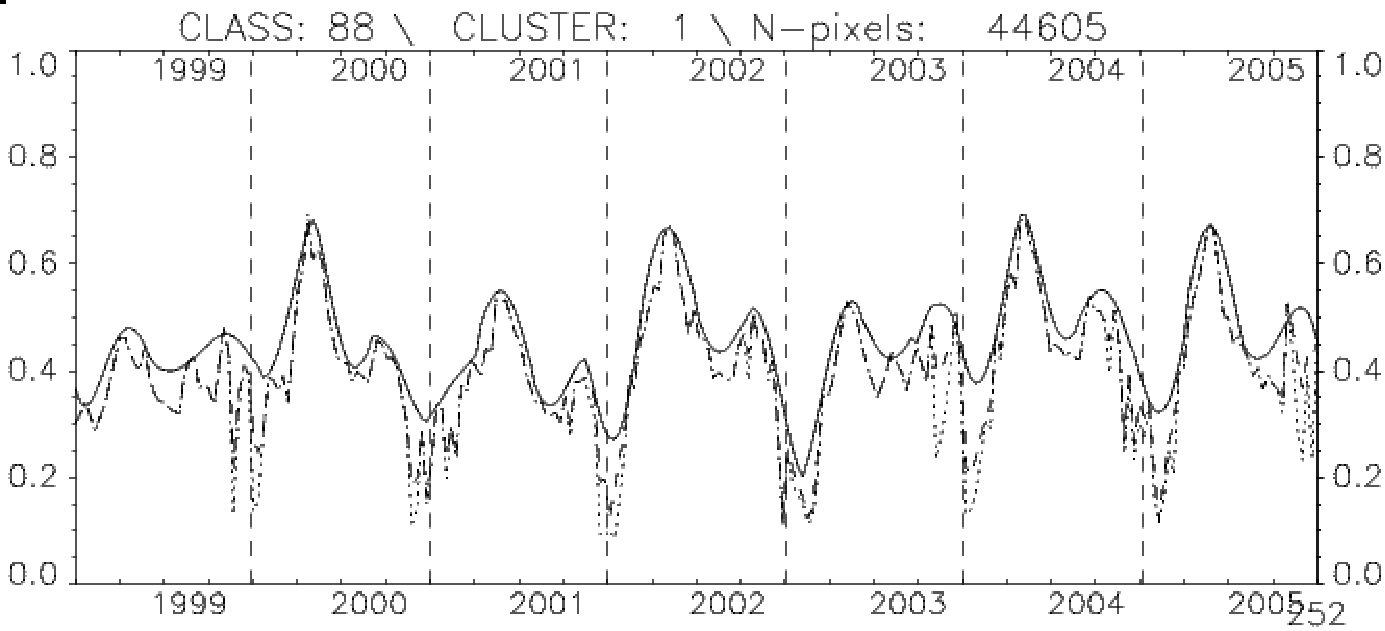
\includegraphics[scale=0.7]{\EPSDIR/plot.pdf}
\caption{\label{figure1} Example of NDVI profiles: rough (dotted), masked (dashed), smoothed (solid). 
(A technical error led to NDVI values overestimated of 0.09 but it has no impact on classification which is relative). }
\end{center}
\end{figure}

In Ecoclimap-II, NDVI satellite data come from SPOT/VEGETATION\footnote{http://free.vgt.vito.be/, http://www.spot.vegetation.com}. 
They are decadal, at true 1-km resolution, that 
is to say that, contrary to AVHRR, one pixel signal is theorically not contaminated by pixels around. Data range from 1999, january to 2005, december.\\ 
They are delivered with a mask encoded on 8 bits: 2 bits represent the situations: clear sky, shadow, uncertain, cloud; 
1 bit for snow and ice, 
1 bit for the land sea mask, and the 4 last bits for the quality of the 4 satellite radiometric bands. This mask is applied in order to keep clear sky 
pixels for which the quality of bands B2 (red) and B3 (near infrared) is good. The land/sea/snow distinction is set by to the classification.\\ 
The plots of NDVI mean profiles for the covers of the C76 map show that data, even if cleared from aberrant values by the mask, remain noisy. 
That's why a smoothing is realized at the upper envelope of the rough curve because highest values are supposed better because atmospheric parameters 
(clouds, water vapor, aerosols) are likely to attenuate the signal reflected to the satellite. Anyway the work on NDVI time series is relative and 
the exact NDVI values don't matter. The smoothing is based on a 4-degree polynomial. 
The figure \ref{figure1} shows effects of the mask and smoothing on the mean NDVI signal for a given class. The distance between the rough and the 
smoothed curves is relative to this mean: the smoothing is done pixel by pixel, filtering out low values entering the mean in the rough case. 

\subsection{The automatic classification process}\label{classif}

The classification algorithm is \textbf{k-means}. 
It consists in reading the NDVI profiles of all pixels of one class, then of gathering closest profiles 
according to the Euclidian distance. Initial center-profiles of clusters are randomly defined and successive iterations are 
performed: each pixel is linked to the most like-looking center-profile; centers of clusters are recalculated; pixels are linked to 
the most like-looking center-profile again, and so on. It's thus necessary to fix from the beginning the number of wished clusters by class.\\ 
A first map is realized by setting high numbers of clusters by classes, then looking at NDVI profiles and geographic positions of the clusters, and 
setting new lower numbers of clusters, until a satisfying classification is obtained. This first map comprises 464 classes and is called \textbf{C464}. \\ 
However, for practical purposes, this method poses several problems: 
\begin{itemize}
\item{When each class of C76 is split into several clusters, the total number of classes increases very fast, rendering 
reading, interpretation and processing hard; }
\item{it boils down to consider initial classes as frozen and separated each from one another, what can prove false, notably with various 
initial maps;}
\item{the continuity of analysis is compromised and the quality of NDVI as classification criterion is hard to evaluate. Moreover, 
numbers of clusters have no option but being arbitrarily posed. }
\end{itemize}
Owing to all these reasons, NDVI is no longer used as a secondary classification criterion: it's admitted that it can rival the initial 
C76 classes boundaries. Moreover, three quantities are now taken into account during the NDVI classification:
\begin{itemize}
\item{the Euclidian distance between profiles (still);}
\item{the correlation between profiles, focusing on the shapes of profiles;}
\item{a criterion mixing the two precedents: $\frac{euclidian~distance}{correlation^{2}}$, outlining the shapes of profiles without neglecting 
the distance between them.}
\end{itemize}
The principle is to gather profiles using a threshold for one or the other of the latter criterions.
Other conditions come then into the picture:
\begin{itemize}  
\item{the size of classes: for example, the threshold is looser for smaller classes, in order not to encourage the formation of low pixels 
number classes;}
\item{the NDVI maximum: as NDVI is the expression of vegetation activity, it's not relevant with low-vegetated areas, also low NDVI maximum 
areas;}
\item{the cover type: water, town and bare soil pixels can't be distinguished through the NDVI, they have to conform the initial nomenclature.}
\end{itemize}
Lastly, comparisons are conducted:
\begin{itemize}
\item{between profiles of clusters and classes they come from: if the cluster is closer to another class than the one it comes from, it can be 
linked to the former class;}
\item{families of classes are formed, then splited in a number of clusters equal to the number of classes constituing them, through the 
automatic classification. Clusters obtained by this totally automatic means are compared to initial classes, in order to verify 
the robustness of the first method through it consistency with the second one. }
\end{itemize}
At each step, the geographic position, the contents of classes according to the initial nomenclature, NDVI profiles and standard deviations 
are observed. These operations allow a better approach of the NDVI time series, adapting to the different types of covers and ensuring more mixing and flexibility than if initial 
boudaries between classes were perfectly respected and if the strict k-means method was applied. 
At this point, the map under construction comprises 257 classes and is called \textbf{C257}. 

\subsection{To the resulting map}\label{end_map}

Several means are added to complete the new map realization:
\begin{itemize}
\item{C257 is compared with the map realized by purely respecting the classes boundaries, C464. 
Every class of each map is splited into 5 clusters through the automatic classification. The distance, the correlation and the standard 
deviation between each cluster and its mother-class are calculated. Maximum, minimum and median of these quantities are compared for C257 and 
C464. Results are equivalent whereas the total numbers of classes clearly vary between the two maps.}
\item{C257 is compared to C76. C76 covers are grouped into 14 general types, close to ISBA vegetation types. Then, each C257 class is divided 
in its contributions to the latter 14 types. Associated NDVI profiles are plotted; geographic distribution of so-obtained clusters is also 
examined. These operations aim at verifying that mixing of initial classes produce consistent and acceptable results. \\
First, given the high resemblance of NDVI profiles of some classes, pixels from a class corresponding to a type (among the 14) that is neither 
its first nor its second prevailing are moved to a class where the considered type prevails, provided that the resemblance between the two classes 
is sufficient (on NDVI profiles). The $\frac{distance}{correlation^{2}}$ criterion is used with a threshold: the moving occurs if the criterion 
is lower than 1., provided that the correlation is positive and higher than 0.9. This operation allows to considerably reduce the distance 
between C76 and C257 in terms of nomenclature. It's also verified that geographically gathered parts of land are not contradictory. Results 
are satisfying. Lastly, on a case by case basis, couple of last reshapings are done. The C257 map becomes at this point \textbf{C271} (with 271 classes). }
\item{NDVI profiles are plotted for only part of the pixels of classes. They are plotted for french pixels and on several specialized classes 
coming from CLC2000: vineyards, orchards, rice fields, olive groves. The goal is to check that those pixels, often melted in larger classes, 
haven't a very particular behaviour that would have been flooded during the classification. This process leads to add still 2 classes of 
vineyards. The final resulting map comprises 273 classes and is called \textbf{C273}. }
\end{itemize}
To conclude, the Ecoclimap-II map comprises 273 classes (see fig. \ref{figure2} for an illustration).  
The classification process combines both an automatic k-means algorithm on NDVI 
seven-years time series from SPOT/VGT and a more or less leaning constraint provided by an initial map built from existing land cover maps 
that are CLC2000 and GLC2000. The nomenclature of this map serves to contain the automatic classification and avoid the emergence of 
incoherent classes. \\
Note also that the use of seven-years time series data induces that the inter-annual variability is taken into account 
during the classification process. 


\begin{figure}
\begin{center}
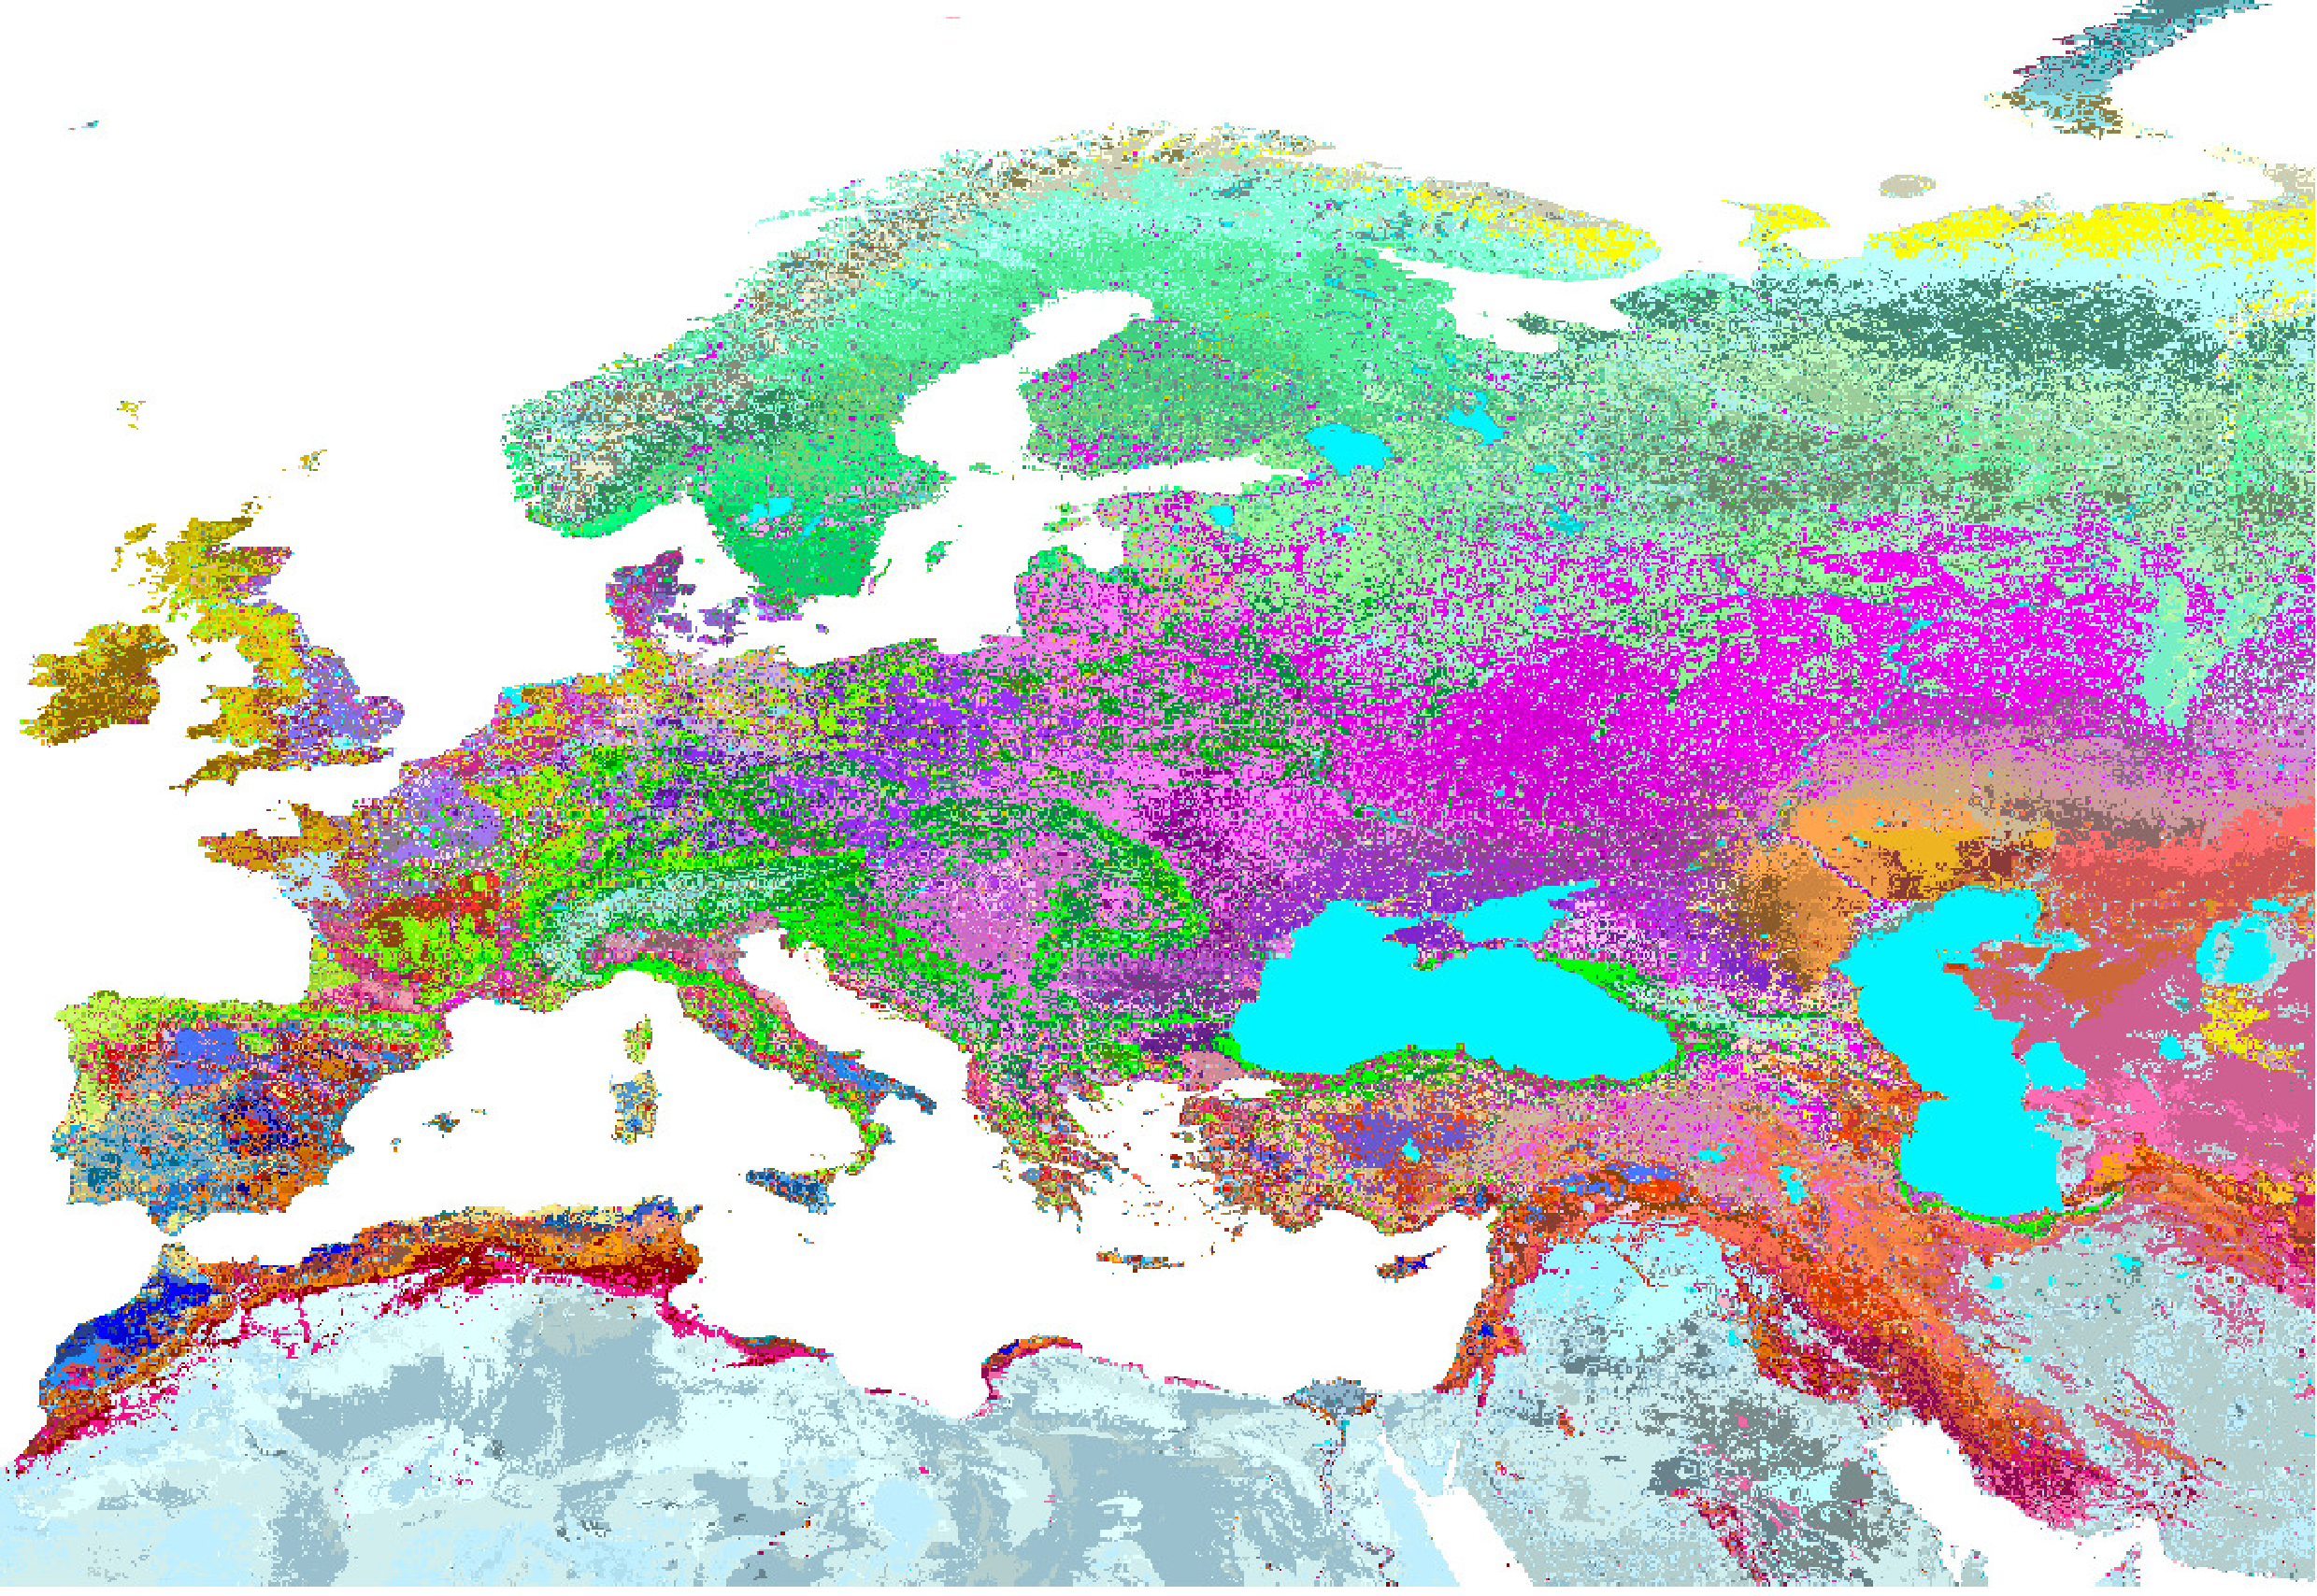
\includegraphics[scale=0.4]{\EPSDIR/europe_eco2.pdf}
\caption{\label{figure2} Ecoclimap-II C273 map on Europe (one color by class) (latlon projection)} 
\end{center}
\end{figure}

\subsection{Short description of covers}

To summarize, it can be said that:
\begin{itemize}
\item{Distribution of forests over the domain is quite linear and progressive, either on the geographic or on the NDVI profiles sides. The evolution 
follows a north-east to south-west axis.}
\item{Crops are very regionalized, in areas with well-marked outlines; they doesn't seem to follow a strictly natural logic. Indeed, 
the human intervention plays a role for these kinds of covers.}
\item{Distribution of shrubs and meadows is intermediate between forests and crops.}
\item{Concerning bare land, snow, inland water and urban areas, resulting classes are very close to those of the initial map C76. Indeed, the NDVI 
classification doesn't allow to discriminate such types of covers. However, the analysis of NDVI profiles is efficient to separate pure 
pixels from mixed ones, and to classify areas functions of the vegetation part of mixed ones. Nevertheless, maintaining such distinctions 
generates a very important amount of classes. That's why only few of these nuances are really integrated in C273, much with bare land and 
snow, just a little with inland water, not at all with urban areas. It could be interesting in the future to study the relevance of such 
distinctions.}
\end{itemize}
Generally, ecosystems are rather homogeneous on large areas in the north continental, and very mixed in the mediterranean perimeter. \\

For practical purposes, it can be noted that classes are numbered from 301 to 573; sea and oceans present in the European domain 
take the number 1 from Ecoclimap-I. 

\section{Translation of covers in tiles and vegetation types}

The next step is to define every new cover as a linear combination of the 4 tiles (types of surface) and the 12 vegetation types (inside 
the "nature" tile). The available sources are following:
\begin{itemize}
\item{(a) Nomenclatures at 1-km resolution from CLC2000, GLC2000 (world, Europe, North Eurasia, Asia, Africa), Ecoclimap-I, C76 (initial map for the classification, see \ref{init_map});}
\item{(a)' The nomenclature at 100m resolution from CLC2000;}
\item{(b) Agricultural statistics from Agreste on France, expressed in hectares, available department by department, since 1989. They comprise 
details about the types of crops;}
\item{(c) a global map about the distribution of C4 vegetation, at 1-degree resolution, provided within the framework of ISLSCP2 and dating from 2003;}
\item{(d) estimates of farm produce by european state, from the FAO;}
\item{(e) data on the maize production by european country in 2003, available on website Ma\"{i}sadour, in thousands of hectares.}
\end{itemize}
The method is then the following:
\begin{itemize}
\item{(a) each Ecoclimap-II cover is broken up among classes of considered other maps. Percentages of representation of the second in the first 
are listed and associated to the titles of the corresponding nomenclatures. The total percentage of the Ecoclimap-II cover in the considered 
map is indicated (in the case of Corine and GLC regional tiles, only a part of the domain is concerned). }
\item{(b) For AGRESTE, department by department, quantities of forests, meadows, C3 crops, C4 crops, permanent crops and other types of covers 
are calculated. Values are averaged on the 1999-2006 spell of time. Resulting curves are plotted and overlain with the associated Ecoclimap-II 
curves, functions of the way of repartition of the covers in the 12 vegetation types.}
\item{(c) The Ecoclimap-II C4 map is resampled at 1-degree resolution in order to compare with the ISLSCP2 map.}
\item{(d) (e) The FAO and Ma\"{i}sadour estimates haven't been exploited yet. }
\end{itemize}
If the class is included in the CORINE area at more than 50\%, the CORINE 100-m information is favoured, instead of 1-km nomenclatures. Amounts of 
C4, C3, meadows, forests, permanent crops are calibrated thanks to the AGRESTE curves, for well-represented classes on France. The ISLSCP2 
map allows to give an idea about the C4 distribution outside France. Note that Agreste provides informations on irrigated surfaces that 
haven't been exploited yet.


\section{Initialization of LAI profiles and other parameters}

In Ecoclimap, as seen in tab. \ref{tab4a} and tab. \ref{tab4b}, several parameters are initialized at the cover level. 

\subsection{Initialization of heights of trees, ground depths, irrigation and town parameters}

First of them, heights of trees are set by using Ecoclimap-I values and the compositions of Ecoclimap-II covers 
into other nomenclatures (GLC, CLC, Ecoclimap-I). Concerning shrubs classes, a distinction is done between meadows 
and low-level trees.\\ 
Then, the ground depths are set by using exclusively the Ecoclimap-I information, the only available. \\
These two last parameters would gain by benefiting from other sources of information.\\ 
Then, the vegetation type "irrigated crops" is arbitrarily considered as composed of C4 crops only. 
In Surfex, the modelling of irrigation passes by four parameters (cf tab. \ref{tab2a}): SEED, REAP, WATSUP and IRRIG. In Ecoclimap-I, 
by default these variables take constant values that are respectively: 10/05, 01/08, 30 and 1. In Ecoclimap-II, these 
default values are kept and defined as soon as the "irrigated crops" fraction is not null. It would be worth leaning on these values 
and precise them according to the classes. \\
Lastly, town parameters don't change in Ecoclimap-II: Ecoclimap urban 
classes are the same in the two versions and come directly from the CLC nomenclature. 

\subsection{Initialization of LAI}

The LAI (Leaf Area Index) is defined as the ratio of total upper leaf (or needle) 
surface of vegetation divided by the surface area of the land on which the vegetation grows. The effective LAI seen by the satellite 
is not the same as the in-situ LAI used by ISBA: the latter is measured on the whole thickness of the vegetation whereas the satellite 
sees only the top of canopy and deduces the LAI by more or less performing algorithms. It notably often causes saturations 
for high LAI. 

\subsubsection{LAI by cover}

Two satellite LAI have been examined for Ecoclimap-II: CYCLOPES (SPOT/VEGETATION) and MODIS. Algorithms leading from the satellite bands 
to the LAI are complex. Land cover maps are included, and the 7 satellite bands (in the case of SPOT) are used. CYCLOPES data range 
from 2000, January to 2004, December; MODIS data from 2000, March to 2006, December. As for the NDVI (see \ref{ndvi}), 
a smoothing by pixel at the 
upper envelop of the LAI profiles is performed. This smoothing is debatable because it makes average LAI values by class very higher 
than these of rough LAI. \\
MODIS LAI, CYCLOPES LAI and SPOT/VGT NDVI are plotted by cover so as to be compared. The three 
products are quite correlated, but MODIS LAI values tend to be higher on forests. Given that 
MODIS LAI time series are longer and that higher values on forests seem more realistic, MODIS LAI are kept 
for Ecoclimap-II. Nonetheless, preconceptions relative to the smoothing could lead in the future to review this LAI and its 
range of values in particular, all the more because tests of smoothing with varying parameters give clearly different results. \\
Moreover, there is a mask with MODIS data that distinguishes not classed data, built areas, wetlands and marshes, permanent 
snow, ice and tundra, bare soil or sparse vegetation areas, inland water, missing data. These masked values can be interpolated in the time 
series, excluded or replaced by zero during the smoothing. It happens that missing data are very numerous at the end of 2000 and 2001, 
particularly for northern and continental classes. That's why, finally, LAI times series are kept only from 2002, January, in order not 
to damage average on all years. It appears necessary to replace masked values because of snow, bare soil or water by zero, since 
LAI are otherwise not realistic (what is seen during the disaggregation coming next). On the contrary, missing and not classed values are interpolated 
in the limit of 4 successive decades, but those which are not interpolated are ignored during the calculation of means by cover 
(acceptable insofar as they are not predominant). 


\subsubsection{Disaggregation of LAI by vegtype inside covers}

\begin{table}[h]
\begin{center}
\begin{tabular}{|l|l|l|l|l|l|l|l|l|l|l|l|l|}
\hline
 & \multicolumn{10}{|c|}{\textbf{fraction of vegetation type}} \\
\hline
\textbf{vegtype} & 90-100\% &  80-90\% & 70-80\% & 60-70\% & 50-60\% & 40-50\% & 30-40\% & 20-30\% & 10-20\% & 0-10\% \\
\hline
CONI & 0 &  6  & 3  & 1  & 3  & 2  & 4  & 4 & 13 & 65 \\
\hline
TREE  & 0 &  2 &  0  & 0 &  1 &  2  & 3 &  6 & 26 & 60 \\
\hline
EVER  & 0  & 0  & 0 &  0  & 0  & 0  & 0 &  0 &  0 &  0 \\
\hline
GRAS  & 0 &  1 &  4 &  2  & 7 & 10 & 14 & 16 & 17 & 29 \\
\hline
TROG  & 0  & 0  & 0  & 0  & 0  & 0 &  0  & 0  & 0 & 100 \\
\hline
PARK  & 9 &  2 &  0 &  0 &  2 &  0 &  2 &  0  & 3 & 83 \\
\hline
C3  & 0  & 1 &  5  & 9  & 9  & 5  & 9 &  5 & 13 & 45 \\
\hline
C4  & 0 &  0 &  1 &  1 &  0 &  1 &  0 &  0 &  2 & 95 \\
\hline
IRR  & 0 &  3  & 5  & 3  & 0  & 2 &  3  & 2  & 2 & 81 \\
\hline
SNOW & 50 &  0 &  0 &  0  & 0 &  0  & 0 &  0 &  0 & 50 \\
\hline
NO  & 3  & 2 &  3 &  4 &  6 &  8 &  6 & 11 & 22 & 35 \\
\hline
ROCK  & 2  & 0  & 0 &  0  & 0 &  0  & 1 &  5  & 7 & 85 \\
\hline
total & 1  & 2 &  3  & 2 &  4 &  4 &  6 &  7 & 15 & 57 \\
\hline
\end{tabular}
\end{center}
\caption{Percentages of classes (calculated functions of the total numbers of classes by vegetation type) concerned by 
the fraction (columns) of each of the 12 vegetation types (lines)}
\label{tab10}
\end{table}

\begin{table}[h]
\begin{center}
\begin{tabular}{|l|l|l|l|l|l|l|l|l|l|}
\hline
\textbf{nb of vegtypes or tiles n} & 1 & 2 & 3 & 4 & 5 & 6 & 7 & 8 & 9 \\
 \hline
\textbf{nb of classes (vegtypes)} & 13  & 6  & 19 & 44 & 45 & 72 & 44 & 23 & 6 \\
\hline
\textbf{nb de classes (tiles)} & 126 & 94 & 53 & 0 & / &  / &  / &  / & / \\
\hline
\end{tabular}
\end{center}
\caption{Number of classes comprising n vegetation types (second line) or n tiles (third line)}
\label{tab11}
\end{table}


Remains to determine LAI by vegtype inside covers from LAI by cover. Given the complexity of classes in terms of vegetation types composition 
(see tab. \ref{tab10} and tab. \ref{tab11}), an automatic LAI disaggregation technique is welcome. The principle of the 
applied method is the following:
\begin{itemize}
\item{LAI 5-years profiles by cover are averaged in order to obtain the annual mean cycles.}
\item{LAI from vegetation types NO, ROCK and SNOW are supposed null and constant.}
\item{In each class, the main vegetation type is put apart. For each of the minority vegetation types, the LAI profile the closest 
according to the $\frac{distance}{correlation^{2}}$ criterion is searched, provided that it corresponds to a class where this vegetation type is 
majority. }
\item{The profile found is taken from the profile of the initial class, weighted by its representation fraction into the class.}
\item{One all minority vegetation types of the classes are thus processed, residual profiles of classes are obtained. Divided by 
the inverse of the fraction of the majority vegetation type, they are admitted to represent the pure majority profiles, in 
the classes.}
\item{The whole operation is repeated, replacing initial classes profiles by the previously obtained pure profiles.}
\item{A new set of pure profiles results, for majority vegetation types of classes. Plotting shows that the three profiles, initial 
(mixte), pure (first extimate), pure (second estimate) differ not much from one another. }
\item{Lastly, 5-years LAI profiles are built by propagating the error between years and the average on the obtained pure profiles.}
\end{itemize}
This method presents two problems: 
\begin{itemize}
\item{The seeking of approached classes only relies on profiles and not on the geographic localisation. Associations of classes coming 
from totally different climate areas are so expectable.}
\item{The technique of subtracting the secondary profiles to deduce the main profile might produce negative LAI.}
\end{itemize}
The first problem is corrected by introducing two climate maps (Firs on Europe, Koeppe et de Lond on the rest of the world). In the 
algorithm above, climate proximity is now favoured with the seeking beginning in the most represented climate area, next the second, etc. 
The second problem is solved by excluding a profile if its subtraction give negative values of LAI. If no suitable profile is found, this which gives 
the less negative values is linearly transformed in order to keep values just over zero. \\

This method presents the advantages that it relies only on the LAI profiles of covers, and doesn't create theoritical profiles. It's fast and 
supple (the longer step is to verify the spatial coherence of the origins of majority and minority profiles) and can be reprocessed 
in case of modifications of the distribution of classes among the 12 vegetation types. It ensures to diversify vegetation types profiles 
inside covers and guarantees the exact reconstitution of LAI covers profiles. However, it should be evaluated if the initial approximation 
between the cover profile and the main vegetation type profile doesn't produce too much bias in the definition of supposed pure profiles. 
But before, MODIS LAI also need to be validated.

\section{Study of the discontinuity at the limits of the domain}

For practical purposes, if the work area overflows the Ecoclimap-II domain, C273 is completed at its edges by Ecoclimap-I. First, north and major part 
of west of the 
domain, there is nearly only sea and ocean (apart from in New-Zemble, but the snow class Ecoclimap-II continues there in the snow class 
Ecoclimap-I). South and a little west, the boundary is located in the Sahara desert. Except from a possible discontinuity between bare rock and bare soil, 
and between very sparse vegetated and desert areas, 
the impact is so minor. Remains the East to study: from northern Russian tundra to Central Asia deserts, by Russian forests, it's 
about quite homogeneous areas organized with latitude, what already dulls the discontinuity.\\
Classes, LAI by class and by vegetation type and vegetation types fractions on both sides are compared. Ecoclimap-II 
classes generally continue in Ecoclimap-I classes. LAI and fractions are often different, but these discrepancies are rarely 
enormous. \\
It's so chosen to begin tests with the straight discontinuity. Then, if the delimitation is too obvious, 
it will be possible to contemplate a version with a smoothed (but artificial) delimitation. 

\chapter{Validation elements for Ecoclimap-II}

Validation aspects relate to three fields: 
\begin{itemize}
\item{Ecoclimap-II new map has already been quite examined during the processing, through comparisons with 
other existing land cover maps (GLC, CLC, Ecoclimap-I - see \ref{classif} and \ref{end_map}). Other tests could be performed, for 
example a comparison with GlobCover, a global land cover map for the year 2005-2006 using ENVISAT MERIS 
fine resolution (300m) data, developed by ESA (European Spatial Agency) and distributed by Medias-France.}
\item{Vegetation types fractions have been set in the light of existing land cover map nomenclatures. Other comparisons 
have been realized with AGRESTE and ISLSCP2 to calibrate values, but also a posteriori with Formosat on a square 
of 60km at the south-west of Toulouse, France. Formosat describes the land cover, year by year, on this area; 
the resolution is 20m. This map is produced by the CESBIO\footnote{Centre d'Etudes Spatiales de la 
BIOsphere (spatial study of the biosphere center)}. This last comparison gives encouraging results but also 
reveals the difficulty of different sources to agree: sources are sometimes contradictory, 
their charasterics and the geographic precision vary and are not necessarily easy to compare. However, 
the progressive use of more recent sources should allow to still refine this definition. Concerning 
specialized vegetation types thar are C4 crops, tropical grassland, irrigated crops, a lack of 
homogeneity inside the covers doesn't allow to get precise fractions. It could be interesting to 
make a potential new map with covers built by introducing entering informations about such characteristics. }
\item{Difficulties have been met to validate other parameters initialized at the cover level: heights of 
trees, ground depths, LAI profiles and irrigation parameters. Indeed, complete and reliable sources 
aren't available. A prospect for the following is thus to find means of validating these quantites. Note again that 
the organization by covers yields a constraint (especially for irrigation) whose reliance could also be interrogated in the light 
of such new validating data. }
\end{itemize}


\chapter{Conclusion}

Ecoclimap-II keeps the same general structure as Ecoclimap-I but several points have changed:
\begin{itemize}
\item{The new covers relie on a k-means automatic classification process and on recent existing land 
cover maps (GLC2000, CLC2000);}
\item{The vegetation types fractions and other cover-based parameters are consequently re-initialized, with 
help from several information sources (AGRESTE, ISLSCP2, land cover maps nomenclatures);}
\item{The LAI profiles by cover come from MODIS satellite data, they are smoothed pixel by pixel;}
\item{The LAI profiles by vegetation type inside covers are built through an original automatic disaggregation 
process in which only LAI profiles by cover step in; }
\item{LAI profiles are available for the average of 5 years (2002-2006) or for each of these years. }
\end{itemize}
Except from these discrepancies, other surface parameters are still likewise obtained. The geographic and 
by patch aggregation also remains. 
Several comparisons with other products have already been done but Ecoclimap-II now needs to be used in 
order to better qualify improvements and wastes in relation with the first version. Further evolution of the database 
is considered functions of users returns and of potential newly available validation data. 

%====================
\bibliography{surfex_scidoc}
%====================
